\documentclass{beamer}

\usepackage{graphicx}
\usepackage{hyperref}
\usepackage{amsmath}

\usetheme{Darmstadt}
\usefonttheme[onlylarge]{structurebold}
\setbeamerfont*{frametitle}{size=\normalsize,series=\bfseries}
\setbeamertemplate{navigation symbols}{}

\usepackage{tikz}
\usetikzlibrary{arrows,shapes}
\usetikzlibrary{calc,decorations.pathmorphing,patterns}
\tikzstyle{block}=[draw opacity=0.7,line width=1.4cm]

%I got the next chunk here https://tex.stackexchange.com/questions/109159/crossing-out-whole-slide-with-latex-beamer as a 
%solution for putting a big x across the whole slide
\makeatletter
\pgfdeclaredecoration{penciline}{initial}{
    \state{initial}[width=+\pgfdecoratedinputsegmentremainingdistance,auto corner on length=1mm,]{
        \pgfpathcurveto%
        {% From
            \pgfqpoint{\pgfdecoratedinputsegmentremainingdistance}
                            {\pgfdecorationsegmentamplitude}
        }
        {%  Control 1
        \pgfmathrand
        \pgfpointadd{\pgfqpoint{\pgfdecoratedinputsegmentremainingdistance}{10pt}}
                        {\pgfqpoint{-\pgfdecorationsegmentaspect\pgfdecoratedinputsegmentremainingdistance}%
                                        {\pgfmathresult\pgfdecorationsegmentamplitude}
                        }
        }
        {%TO 
        \pgfpointadd{\pgfpointdecoratedinputsegmentlast}{\pgfpoint{8pt}{5pt}}
        }
    }
    \state{final}{}
}

\newcommand{\var}{{\operatorname{var}}}
\newcommand{\cov}{{\operatorname{cov}}}
\newcommand{\cor}{{\operatorname{cor}}}
\newcommand{\E}{{\operatorname{E}}}
\newcommand{\mean}{{\operatorname{mean}}}
\newcommand{\cosp}{{\operatorname{cosp}}}

% ------------------------------------------------------------------------------
% got this from here: https://www.overleaf.com/latex/examples/code-presentations-example-different-ways-shown-in-beamer-metropolis/tsxpnyjbhbds
% ------------------------------------------------------------------------------
\let\textttorig\texttt
\renewcommand<>{\texttt}[1]{%
  \only#2{\textttorig{#1}}%
}

\title[Wavelet approaches to synchrony]
{
wsyn: Wavelet approaches to studies of synchrony in ecology
}

\author[Reuman]
{
D.C.~Reuman\inst{1} \\
J.A.~Walter\inst{2}
}

\institute
{
\inst{1}
University of Kansas \\
\inst{2}
UC Davis and University of Virginia
}

\date[KPT 2003]
{
May, 2024
}

\begin{document}

\begin{frame}
\titlepage
\end{frame}

\section{Introduction}


\section{wsyn and synthetic examples}

%Somewhere above here you need to say the viewpoint is operational, i.e.,
%we talk about what these tools can get you and how you intepret it. Main ideas. 
%No time for detailed math, but we can provide some references if you want. 

%We should probably have a "reference" section in the github where we put:
%1) Torrence and Compo
%2) Some of our papers
%3) The wsyn vignette pdf
%3) A longer reference list

%You also want to mention, Dan, that the codes for this are in the github for the 
%seminar, and these are abbreviated from the vignette, so you have those two 
%resources, the latter in greater depth than what I have time for here.

\subsection{Wavelet transform}

\begin{frame}
\frametitle{How to use the wavelet transform}
\begin{itemize}
\item Given a time series $x(t)$, the wavelet transform, $W_{\sigma}(t)$ is a complex number with:
\begin{itemize}
\item magnitude the strength of oscillation in $x(t)$ at time $t$ and timescale $\sigma$
\item phase the phase of that oscillation
\end{itemize}
\item So it decomposes variation by timescale, and tells you how that changes through time
\item You could also think of it as a time-windowed Fourier transform (but done correctly)
\end{itemize}
\end{frame}

\begin{frame}[fragile]
\frametitle{Example of wavelet transform: make some data}
\begin{block}{Fake data characteristics}
\begin{itemize}
\item One time series, sin wave of period 15, then switches to 8...
\item Plus white noise
\end{itemize}
\end{block}
\begin{exampleblock}{Make some fake data}
\begin{verbatim}
time1<-1:100; time2<-101:200; times<-c(time1,time2)

ts1<-c(sin(2*pi*time1/15),0*time2) #starts period 15
ts2<-c(0*time1,sin(2*pi*time2/8)) #then period 8
ts3<-rnorm(200,mean=0,sd=0.5) #add some white noise

ts<-ts1+ts2+ts3 
\end{verbatim}
\end{exampleblock}
\end{frame}

\begin{frame}[fragile]
\frametitle{Example of wavelet transform: apply \texttt{wsyn::wt}}
\begin{exampleblock}{Apply \texttt{wt}}
\begin{verbatim}
ts<-wsyn::cleandat(ts,times,clev=1)$cdat
wtres<-wsyn::wt(ts$cdat,times)
\end{verbatim}
\end{exampleblock}
\begin{block}{Notes}
\begin{itemize}
\item \texttt{cleandat} demeans time series (can also do more)
\item \texttt{wtres} is an S3 class defined for wavelet transforms
\item Default values for other \texttt{wt} arguments are good for exploration
\end{itemize}
\end{block}
\end{frame}

\begin{frame}[fragile]
\frametitle{Example of wavelet transform: what do you get?}
\begin{exampleblock}{Plot magnitude and phase}
\begin{verbatim}
wsyn::plotmag(wtres)
wsyn::plotphase(wtres)
\end{verbatim}
\end{exampleblock}
\includegraphics[width=.49\textwidth]{../results/synthetic_results/WaveletExample_magnitude.pdf}
\includegraphics[width=.49\textwidth]{../results/synthetic_results/WaveletExample_phase.pdf}
\end{frame}

\begin{frame}
\frametitle{Wavelet transform example}
\begin{columns}[c]
\begin{column}{6cm}
\begin{itemize}
\item The wavelet magnitude shows periodicity and change therein
\item A power spectrum would just show two peaks at timescales 8 and 15, no time resolution
\end{itemize}
\end{column}
\begin{column}{6cm}
\includegraphics[width=\textwidth]{../results/synthetic_results/WaveletExample_magnitude.pdf}
\end{column}
\end{columns}
\end{frame}

\subsection{Two ways to show time- and timescale-specific synchrony}

\begin{frame}
\frametitle{The wavelet phasor mean field (\texttt{wsyn::wpmf})}
  \begin{itemize}
    \item For timeseries $x_n(t)$ in $n=1,\ldots,N$ locations
    \item For wavelet transforms $W_{n,\sigma}(t)$
    \item The WPMF is $\frac{1}{N} \sum_n \frac{W_{n,\sigma}(t)}{|W_{n,\sigma}(t)|}$
    \item In other words average the ``phasors'' $p_{n,\sigma}(t)= \frac{W_{n,\sigma}(t)}{|W_{n,\sigma}(t)|}$
    \item A ``phasor'' is a unit-magnitude complex number
    \item It gives phase synchrony as a function of time and timescale
  \end{itemize}
\end{frame}

\begin{frame}
  \frametitle{The wavelet phasor mean field - gives a detailed picture of synchrony}
  \begin{center}
    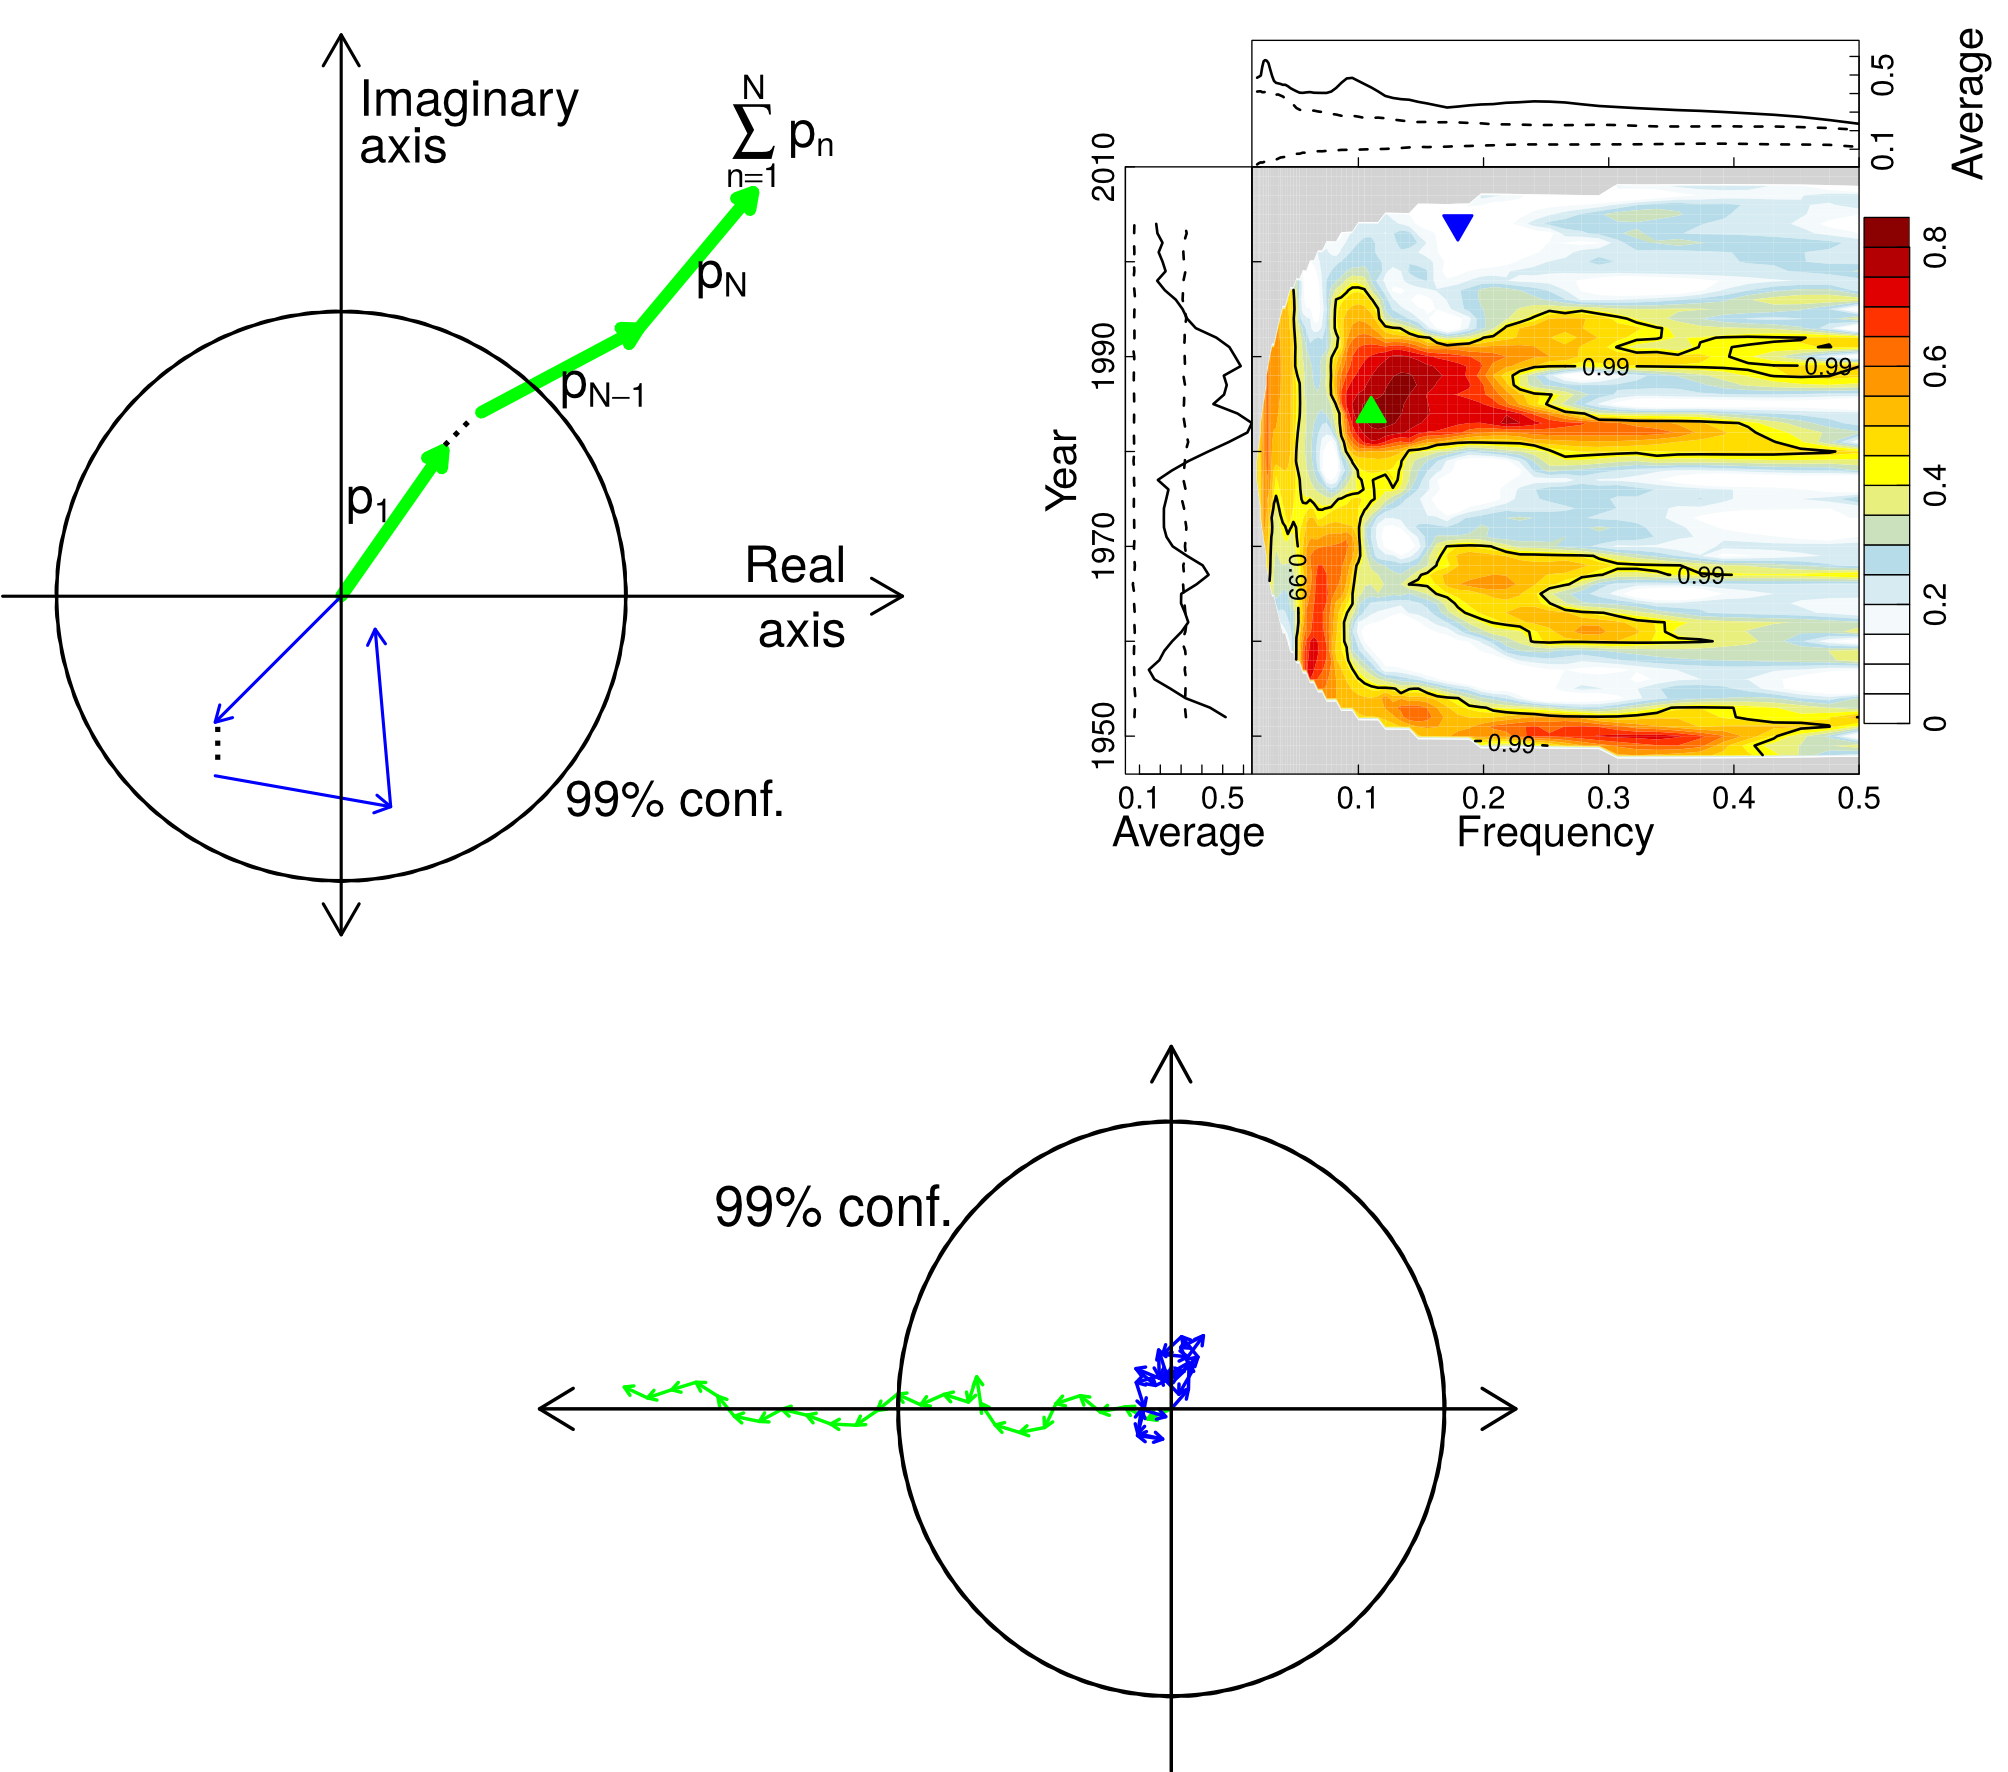
\includegraphics[height=8cm]{./figures/WPMF.png}
  \end{center}
\end{frame}

\begin{frame}[fragile]
\frametitle{Example of the wpmf: make some data}
\begin{block}{Fake data characteristics}
\begin{itemize}
\item Several time series
\item All have one underlyig signal, switches from period 10 to 5 mid way
\item All have randomly phase-shifted period-3 sine ways
\item Plus white noise, independent in each signal
\end{itemize}
\end{block}
\end{frame}

\begin{frame}[fragile]
\frametitle{Example of the wpmf: make some data}
\begin{exampleblock}{Make some fake data}
\begin{verbatim}
times1<-0:50; times2<-51:100; times<-c(times1,times2)
ts1<-c(sin(2*pi*times1/10),sin(2*pi*times2/5))+1.1 

dat<-matrix(NA,11,length(times))
for (counter in 1:dim(dat)[1])
{
  ts2<-3*sin(2*pi*times/3+2*pi*runif(1))+3.1
  ts3<-rnorm(length(times),0,1.5)
  dat[counter,]<-ts1+ts2+ts3    
}
dat<-cleandat(dat,times,1)$cdat
\end{verbatim}
\end{exampleblock}
\end{frame}

\begin{frame}
\frametitle{Can you see synchrony in these data? Not really.}
\includegraphics[width=.49\textwidth]{../results/synthetic_results/WPMFExample_timeseries.pdf}
\includegraphics[width=.49\textwidth]{../results/synthetic_results/WPMFExample_PairwiseCorrelation.pdf}
\end{frame}

\begin{frame}[fragile]
\frametitle{Example of wpmf: apply \texttt{wsyn::wpmf}}
\begin{exampleblock}{Apply \texttt{wpmf}}
\begin{verbatim}
wpmfres<-wsyn::wpmf(dat,times,sigmethod="quick")
\end{verbatim}
\end{exampleblock}
\begin{block}{Notes}
\begin{itemize}
\item \texttt{wpmfres} is an S3 class defined for wpmfs 
\item Default values for other arguments are good for exploration, see docs and vignette for details
\end{itemize}
\end{block}
\end{frame}

\begin{frame}[fragile]
\frametitle{Example of wpmf: what do you get?}
\begin{exampleblock}{Plot magnitude}
\begin{verbatim}
wsyn::plotmag(wpmfres,sigthresh=0.95)
\end{verbatim}
\end{exampleblock}
\begin{columns}[c]
\begin{column}{6cm}
\includegraphics[width=\textwidth]{../results/synthetic_results/WPMFExample_wpmf.pdf}
\end{column}
\begin{column}{6cm}
\begin{itemize}
\item We get significant synchrony at timescale 10, initially, then at timescale 5
\item So we detect the time- and timescale-specific synchrony what was built into the data
\end{itemize}
\end{column}
\end{columns}
\end{frame}

\begin{frame}
\frametitle{Significance of the wpmf}
\begin{itemize}
\item Null hypothesis: random, independent phasors
\item Significance means phasors are significantly more aligned than that
\item Note: as always, you need to keep multiple testing in mind
\end{itemize}
\begin{center}
\includegraphics[width=.5\textwidth]{../results/synthetic_results/WPMFExample_wpmf.pdf}
\end{center}
\end{frame}

\begin{frame}
\frametitle{The wavelet mean field (\texttt{wsyn::wmf})}
  \begin{itemize}
    \item We also use the ``wavelet mean field'' $r_\sigma(t)=\frac{1}{N}\sum_{n=1}^{N}w_{n,\sigma}(t)$
    \item Where $w_{n,\sigma}(t)=W_{n,\sigma}(t)/\sqrt{\frac{1}{NT}\sum_{n=1}^{N}\sum_{t=1}^{T}W_{n,\sigma}(t)W_{n,\sigma}^{*}(t)}$ is a normalized wavelet transform
    \item The wmf uses magnitude as well as phase information, gives more complete information but a bit more complicated
    \item Can interpret it in a similar way
    \item But no straightforward significance testing!
    \item We often show both
    \item See \texttt{wsyn} vignette for details on how to call the \texttt{wmf} function
  \end{itemize}
\end{frame}

\subsection{Wavelet coherence}


\subsection{Attributing synchrony to causes}



\section{Kelp example}






\end{document}